\begin{chapter}{Основная часть}

\section{Постановка задачи}
	\begin{enumerate} 
      \item[1)]  Создание датчиков.
      \item[2)]  Генерация отправки данных на устройства.
      \item[3)] Анализ и обработка данных.
      \item[4)] Создание умных оповещений.
    \end{enumerate}

\section{Общая архитектура системы}

    Для создания проекта использовались платформа Thingsboard и графический конфигуратор для интернета вещей Node-red. Реализация работы выполнена и выложена в репозиторий на  \href{https://github.com/alexeyhorkin/IoT_UNN_HW}{github}, запуск осуществляется с  помошью docker.
    
    \textbf{Thingsboard} - платформа IoT с открытым исходным кодом, через которую происходило управление устройствами, сбор, обработка и визуализация данных.
    
    \textbf{Node-red} - графический конфигуратор, который позволяет через браузер построить схему взаимодействия устройст между собой и внешними системами.
    
\section{Node-Red}

    На изображении мы можем видеть четыре цепочки данных. С помощью них генерируются и отправляются данные о давлении, температурах, местоположении и скорости.
    
    \begin{figure}[!ht]
		\centering
		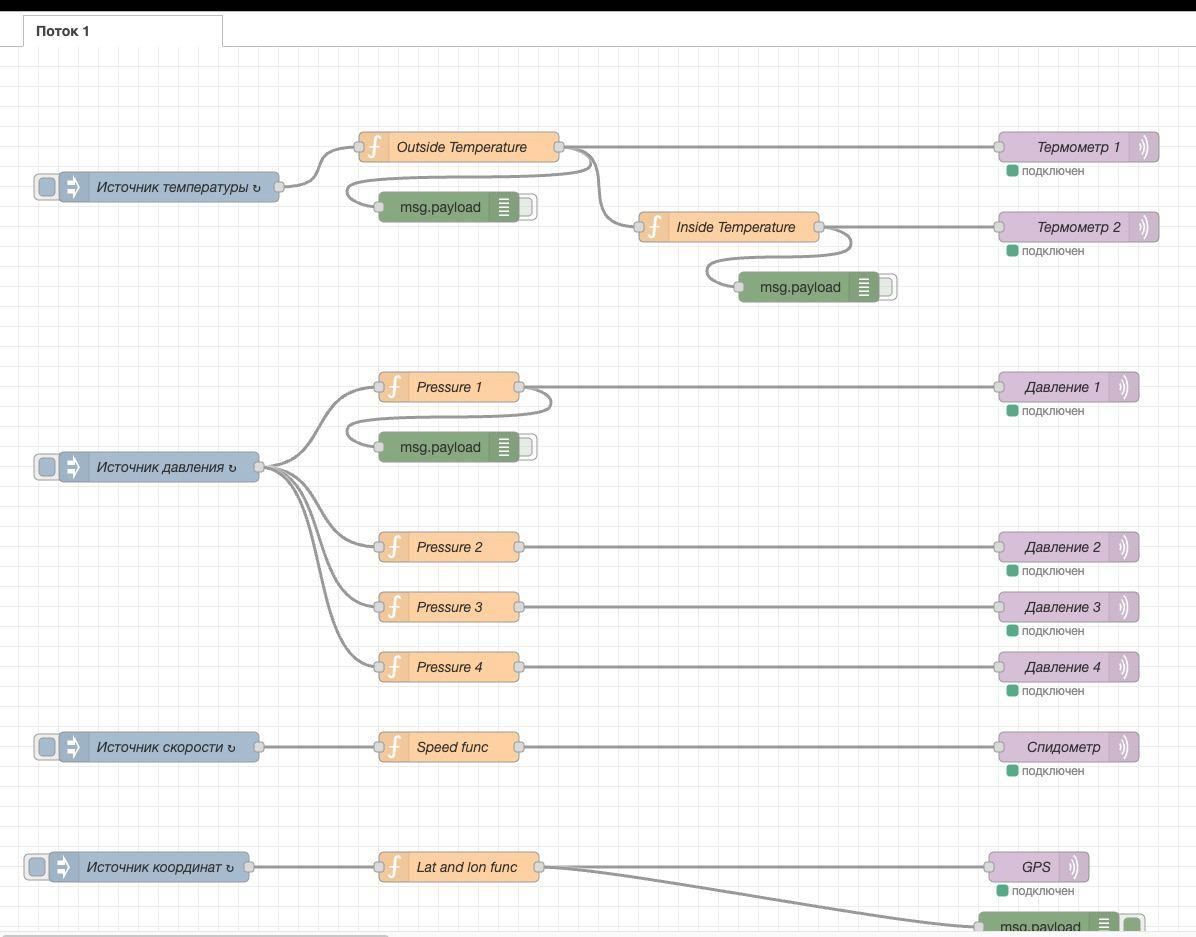
\includegraphics[scale=0.4]{pictures/8.jpg}
		\caption{Node-Red архитектура.}
		\label{fig1}
	\end{figure}
	

\section{Thingsboard}

    Для создания проекта нам потребовались следующие активы: <<Mini Cooper>>, <<Колесо ЗЛ>>, <<Колесо ЗП>>, <<Колесо ПЛ>>, <<Колесо ПП>>. В каждом из них указаны взаимоотношения между собой, при этом образуется иерархия.
    
    Были и созданы необходимые устройства: <<Давление 1-4>>, <<Температура 1-2>>, <<Спидометр>>, <<GPS>>.
    
    \begin{figure}[!ht]
		\centering
		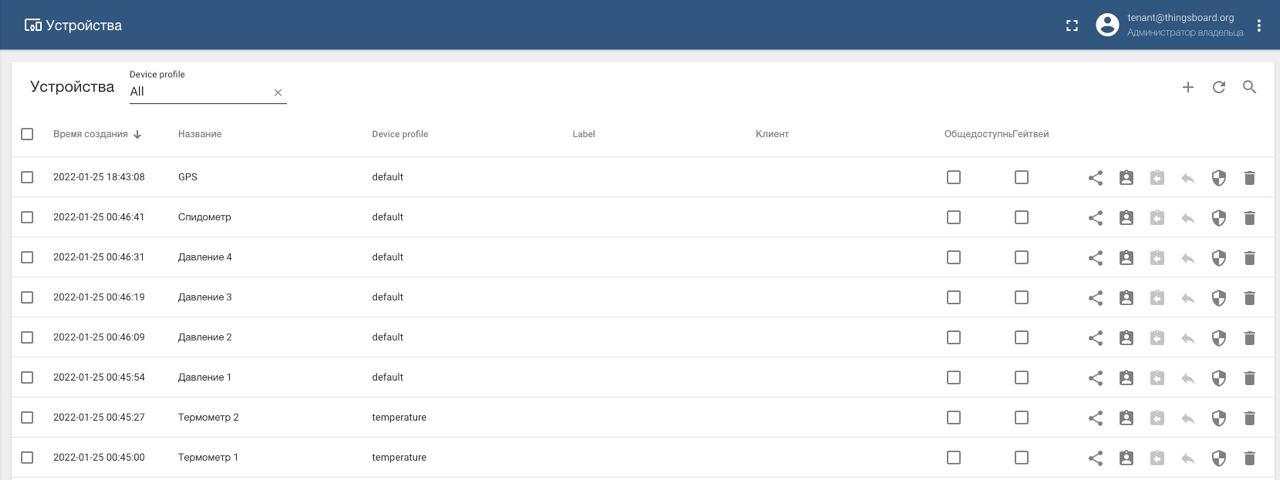
\includegraphics[scale=0.4]{pictures/4.jpg}
		\caption{Используемые устройства в Thingsboard.}
		\label{fig1}
	\end{figure}

    На главном экране дашборда располагаются виджеты:
    
	\begin{enumerate} 
      \item[1)]  Иерархия активов и устройств.
      \item[2)]  Карта с местоположением автомобиля.
      \item[3)]  Виджеты датчиков давления на каждое колесо.
      \item[4)]  Виджет спидометра.
      \item[5)]  Виджеты внутренней и внешней температур.
    \end{enumerate}

    \begin{figure}[!ht]
		\centering
		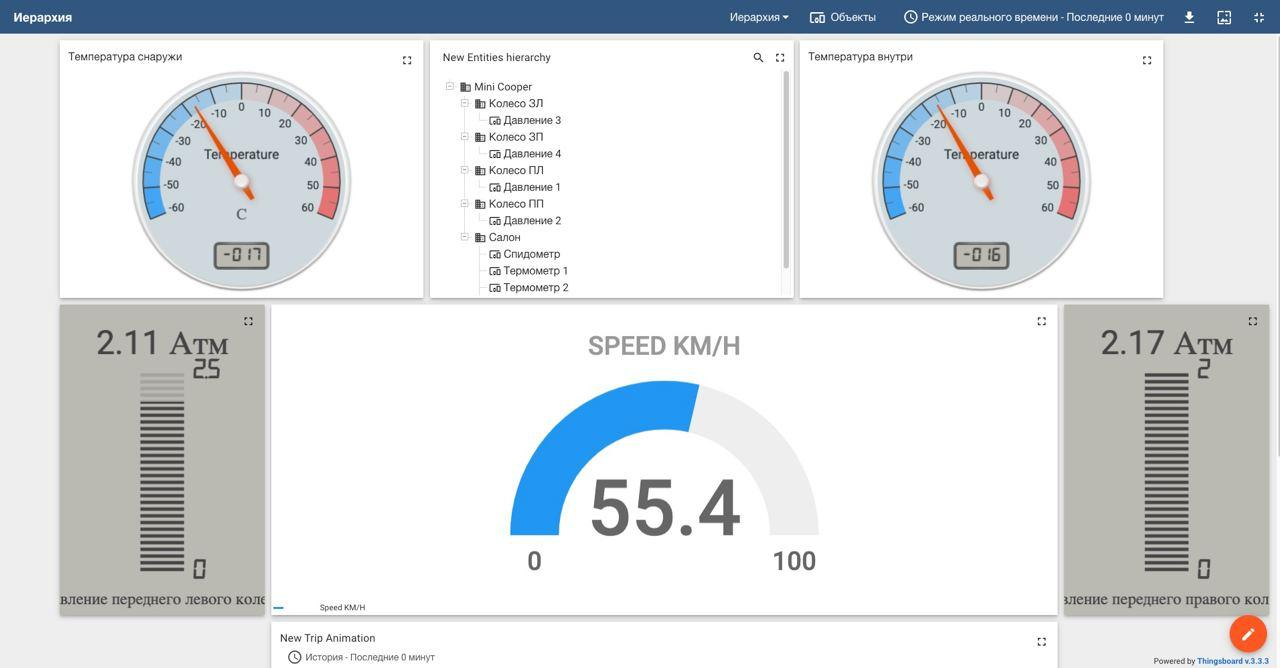
\includegraphics[scale=0.5]{pictures/2.jpg}
		\caption{Виджеты в Thingsboard.}
		\label{fig1}
	\end{figure}

    \begin{figure}[!ht]
		\centering
		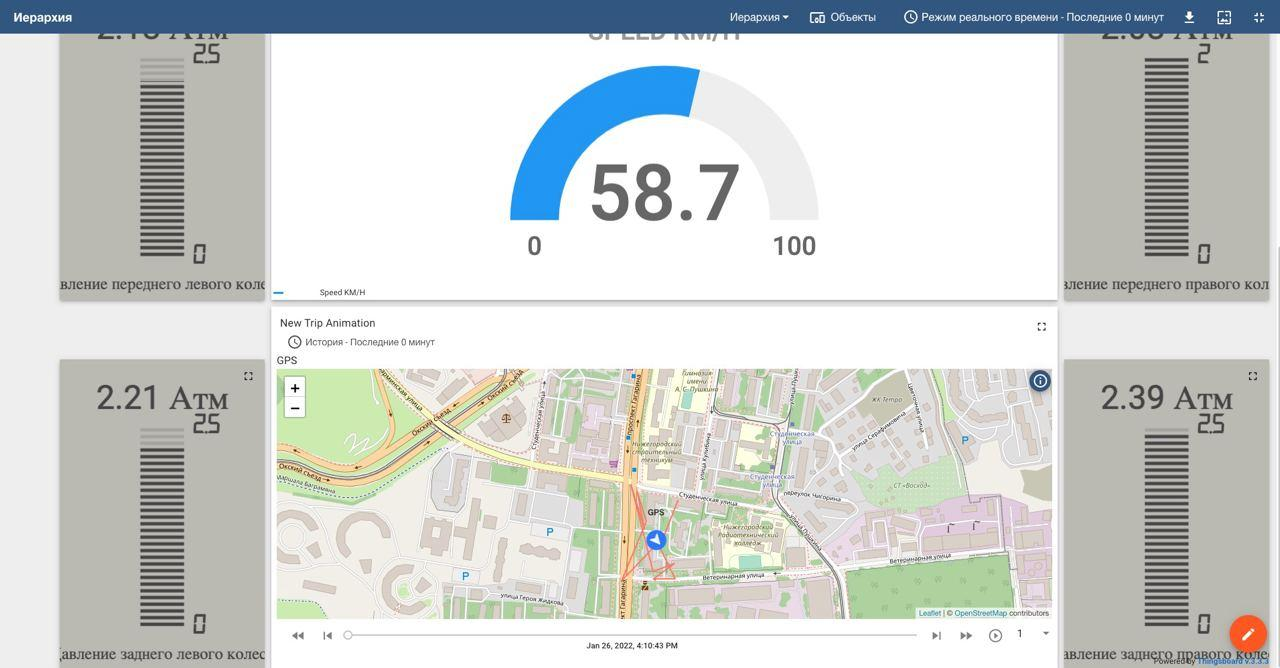
\includegraphics[scale=0.5]{pictures/3.jpg}
		\caption{Виджеты в Thingsboard.}
		\label{fig1}
	\end{figure}
	
В другом дашборде расположена информация о данных датчика внутренней температуры. Информация представлена в следующем виде:

	\begin{enumerate} 
      \item[1)]  График.
      \item[2)]  Оповещения.
    \end{enumerate}
    
    \begin{figure}[!ht]
		\centering
		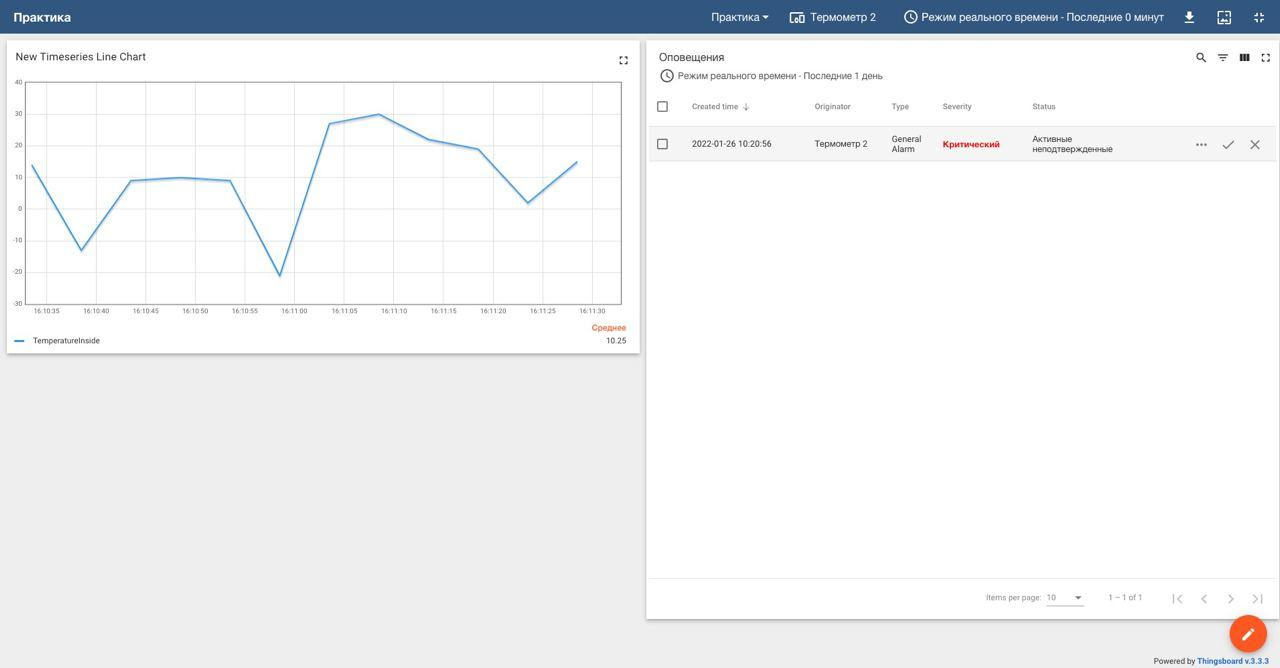
\includegraphics[scale=0.5]{pictures/1.jpg}
		\caption{Виджет графика внутренней температуры в Thingsboard.}
		\label{fig1}
	\end{figure}

Была реализована цепочка для работы датчиков.

\newpage

    \begin{figure}[!ht]
		\centering
		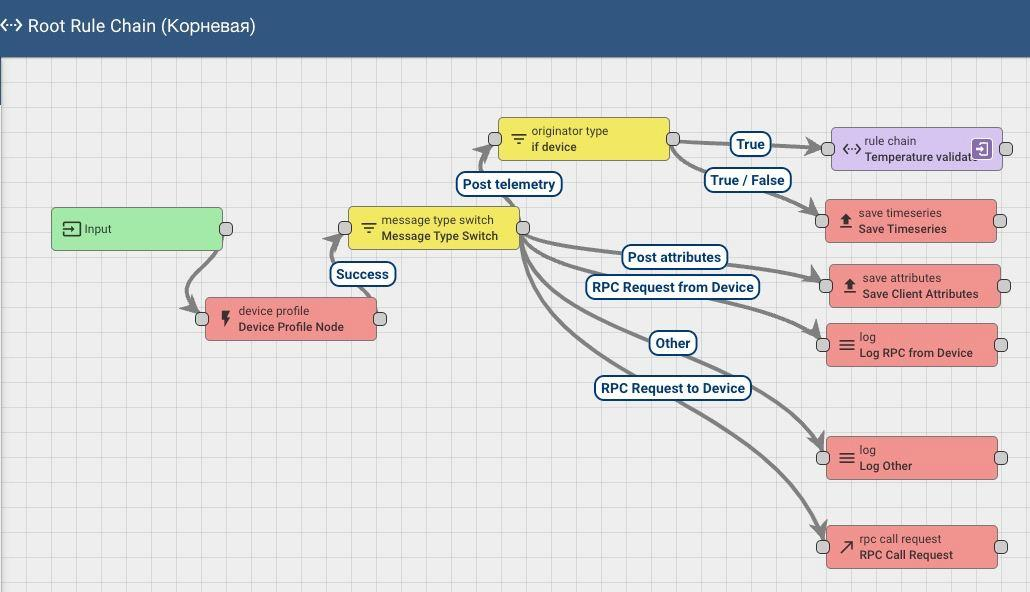
\includegraphics[scale=0.6]{pictures/6.jpg}
		\caption{Цепочка для работы датчиков.}
		\label{fig1}
	\end{figure}


В цепочке валидации температуры мы проверяем, что данные пришли с температурного сенсора, ответственного за температуру внутри салона. Затем, мы извлекаем серверные атрибуты <<maxTemp>> и <<minTemp>> с устройства, на основе которых происходит валидация. И в зависимости от результата создается определенное оповещение, сохраняется телеметрия, а также отправляется уведомление на почту.

    \begin{figure}[!ht]
		\centering
		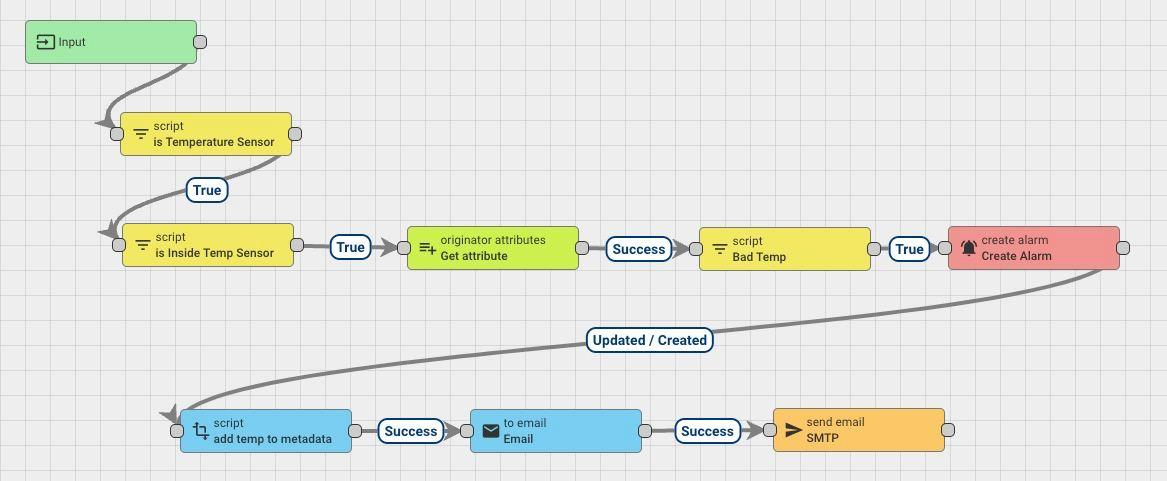
\includegraphics[scale=0.55]{pictures/7.jpg}
		\caption{Цепочка для работы предупреждений.}
		\label{fig1}
	\end{figure}

\newpage
\end{chapter}
